\documentclass{kththesis}

\usepackage[export]{adjustbox}
\usepackage{amsmath}
\usepackage[style=numeric,sorting=none,backend=biber]{biblatex}
\usepackage{booktabs}
\usepackage{caption}
\usepackage{color}
\usepackage{csquotes} % Recommended by biblatex
\usepackage[super]{nth}
\usepackage{float}
\usepackage{relsize}
% \usepackage{siunitx}
\newcommand{\num}[1]{{#1}}
\usepackage{soul}
\usepackage{subcaption}
\usepackage{tabularx}
\usepackage{wrapfig}

\addbibresource{references.bib} % The file containing our references, in BibTeX format
\renewcommand{\arraystretch}{1.2}
\newcommand{\source}[1]{\vspace{-5mm}\caption*{\textcolor{darkgray}{Author: {#1}}\vspace{-7mm}} }
\captionsetup[table]{skip=10pt}
\restylefloat{table}

\title{Evaluating different training techniques for a convolutional neural network that classifies Alzheimer's disease}
\alttitle{Utvärdering av olika träningstekniker för ett CNN-nätverk som klassificerar Alzheimers sjukdom}
\author{Karl Lundstig}
\email{lundsti@kth.se}
\supervisor{Jeanette Hällgren Kotaleski}
\examiner{Örjan Ekeberg}
\programme{Degree Project in Computer Science, DD142X}
\school{School of Electrical Engineering and Computer Science}
\date{\today}

% Uncomment the next line to include cover generated at https://intra.kth.se/kth-cover?l=en
\kthcover{kth-cover.pdf}


\begin{document}

% Frontmatter includes the titlepage, abstracts and table-of-contents
\frontmatter

\titlepage

\begin{abstract}
Effective computer diagnosis of Alzheimer's disease could bring large benefits to the millions of people worldwide who does or will suffer from dementia. One popular method for trying to achieve this is the training of convolutional neural networks to classify MRI brain scans. An abundance of training methods exists that aims to improve the performance of these neural networks, but their effectiveness and eventual disadvantages are not always clear.
  
This study evaluates the performance of a CNN on the OASIS-3 neuroimaging dataset. The CNN's task is to classify each MRI scan into one of four classes which correspond to the stage of Alzheimer's disease. Two different training methods are compared to a training baseline. The first method evaluated is class-weighting, a technique that tries to compensate for rare classes in imbalanced datasets. The second method is data augmentation, a technique that extends the dataset in an attempt to reduce overfitting and increase performance.
  
Class-weighting was found to improve the classification performance significantly on the rarest class, while not having too large effect on the other classes. Data augmentation was not found to improve performance in general, but did improve the recall on some classes.

\end{abstract}


\begin{otherlanguage}{swedish}
  \begin{abstract}
    Effektiv datorbaserad diagnos av Alzheimers sjukdom skulle kunna medföra stora fördelar för de som lider av eller kommer drabbas av demens. En populär metod för att åstadkomma detta är tränandet av konvolutionella neurala nätverk (CNNs) som klassifierar magnetröntgenskanningar av hjärnan. Ett överflöd av träningsmetoder finns som försöker förbättra de här neurala nätverkens träffsäkerhet, men deras effektivitet och eventuella nackdelar är inte alltid tydliga.

    Den här studen undersöker träffsäkerheten av ett CNN på hjärnavbildningsbanken OASIS-3. Nätverkets uppgift är att klassifiera varje MRI-bild som en av fyra klasser, whilka motsvar stadiet av Alzheimers sjukdom. Two olika träningsmetoder jämförs mot en grundmetod. Den första metoden som provas är klassviktning, en teknik som försöker kompensera för ovanliga klasser i en datamängd. Den andra metoden är datautökning, en teknik som utökar datamängded i ett försök att minska överträning och öka träffsäkerheten

    Klassviktning visades tydligt öka klassifieringträffsäkerheten på den ovanligaste klassen, utan att ha alltför stor effekt på säkerheten för de andra klasserna. Datautökning ökade inte träffsäkerheten generallt, men förbättrade täckningen på vissa klasser.
  \end{abstract}
\end{otherlanguage}


\setcounter{secnumdepth}{2}
\setcounter{tocdepth}{2}
\tableofcontents


% Mainmatter is where the actual contents of the thesis goes
\mainmatter

\chapter{Introduction}
In the last couple of years machine learning, and more specifically deep learning, have been applied successfully on a multitude of problems. These problems cover various areas such as speech recognition, image recognition \parencite{krizhevsky2012imagenet}, and even board games \parencite{silver2018general}. One place where effective image recognition and analysis could be applied to great benefit is in the field of medical diagnostics. Computer-aided detection and diagnosis can help physicians interpret medical images, decreasing the time spent on interpretation and possibly even increasing accuracy~\cite{erickson2017machine}.

Dementia is an umbrella term for several diseases affecting memory and cognitive abilities, and in 2015 affected 47 million people worldwide (5~\% of the world’s elderly population). This number is predicted to increase to 75 million by 2050~\cite{dementiaWHO}. The leading cause of dementia is the neurodegenerative \textit{Alzheimer’s disease}. No cure currently exists for this brain disease, but early detection is still important as it carries with it several benefits for the patient~\cite{factsfigures2018}. Alzheimer's causes brain atrophy, which can be detected using MRI imaging. Several studies~\cite{islam2017novel, islam2018early} shows promising results for identifying and classifying Alzheimer’s disease using convolutional neural networks (CNNs) trained on these structural MRI images.

Machine learning is a complex field, and CNNs can be used in a wide variety of ways. They can have different activation functions, different number of layer and filters, and varying depths. The training of a CNN can also be performed in various ways, with different hyperparameters, error functions, and dataset layouts.

\section{Research Question}
Choosing the correct way of training a CNN can have a significant impact on the resulting performance. This study aims to evaluate two training methods that are often used and relevant for CNN models:
\begin{enumerate}
	\item{The use of class-weighting in the error function. This can be applied to alleviate bias when the classes in the dataset are of very different sizes.}
	\item{Data augmentation. This can be used to reduce overfitting and improve performance when datasets are small.}
\end{enumerate}
These methods tries to solve different problems and can each be applied independently to an existing model. They can be useful for all kinds of CNNs, but this study will focus on their effects on Alzheimer's diagnosis using MRI imaging. To this end, a simple CNN will be created, and its performance will be assessed when training, first without any of these methods, then with \textit{class-weighting}, and finally with \textit{data augmentation} and class-weighting. The following questions will be answered:

\begin{itemize}
\item{Does class-weighting improve the performance on rarer classes?}
\item{Does data augmentation improve general performance?}
\end{itemize}

\chapter{Background}

\section{Alzheimer's Disease}

Dementia is a group of symptoms that may have many different causes. One common cause is Alzheimer's disease, a degenerative brain disease that is estimated to occur in 60\% to 80\% of dementia cases. In half of these cases of dementia Alzheimer's is the only cause, while many other also have evidence of other changes to the brain~\cite{factsfigures2018}.
Individuals with Alzheimer's disease may experience multiple symptoms, which may vary over the course of the illness~\cite{factsfigures2018}.

\subsection{Benefits of early detection}
Early (and accurate) diagnosis of Alzheimer's disease has several benefits. Those who do not have Alzheimer's but are diagnosed with mild cognitive impairment, might after testing realize that they're suffering from some other, treatable condition. There are also medical and social benefits to get an Alzheimer's diagnosis early. Neither a curing nor a slowing treatment exist, but individuals can still take some measures that helps them retain their cognitive function for as long as possible. Aerobic exercise, mental activity and social engagement may help delay cognitive decline, while medication and other intervention can help with managing symptoms. An early diagnosis can also help reduce anxiety by giving noticed symptoms a name, for both affected individuals and their family members. Finally, early diagnosis gives individuals time to make plans for the future while still having good cognitive function~\cite[p. 406-409]{factsfigures2018}.

\subsection{Brain changes}
\begin{figure}
  \centering
  \includegraphics[width=0.9\linewidth]{img/mri_scan.png}
  \caption{The three planes of a brain MRI scan.}
\end{figure}
The abnormal accumulation of two proteins (into what is called beta-amyloid plaques and tau tangles) inside the brain is one of several brain changes associated with Alzheimer's disease. These proteins interfere with neuron communication and nutrient transportation, while also triggering inflammation. Brain shrinkage, or \textit{atrophy,} eventually occurs due to cell loss. These protein changes may start as early as 20 years or more before symptoms appear~\cite{factsfigures2018}.

Brain atrophy occurs in a relatively late disease stage, when neurodegeneration has started to occur. This can be detected and measured using MRI imaging. Atrophy is a medically established predictor of an individual progressing from mild cognitive impairment to Alzheimer's disease. In addition, there seems to be a direct relationship between the severity of the atrophy and time-to-dementia. Brain atrophy is nevertheless not a unique sign of Alzheimer's, but a measure of neural degeneration in general. Degeneration might be caused by other conditions~\cite{jack2010brain}.

\subsection{Clinical dementia rating}
Clinical dementia rating (CDR) is a score that is used to classify the stage of Alzheimer’s disease. Scores 0.0 through 2.0 is described in Table~\ref{tab:cdr_definition}. There also exists a final score of 3.0~\cite{cdr}. This score is not relevant to this study, as the disease in this stage is too severe to partake in medical studies.

The CDR is derived from an interview with the patient as well as an informant, where impairment to six cognitive categories are scored: Memory, Orientation, Judgment and Problem Solving, Community Affairs, Home and Hobbies, and Personal Care. The final CDR score is a combination of all the categories, with \textit{Memory} being given extra weight~\cite{cdr}.

\begin{table}[h]
  \renewcommand{\arraystretch}{1.2}
  \begin{center}
    \caption{Clinical dementia rating}
    \label{tab:cdr_definition}
    \begin{tabularx}{\textwidth}{c|cX}
      \textbf{Score} & \textbf{Severity of AD} & \textbf{Description} \\
      \toprule
      0.0 & None & No consistent forgetfulness. Cognitively normal. \\
      0.5 & Very mild & Slight, 'benign` forgetfulness. Slight impairment to problem solving, social activities, and hobbies. Able to fully care for oneself. \\
      1.0 & Mild & Moderate memory loss. More difficult chores and interests abonded. Moderate difficulty with time relationships. Need prompting for personal care. \\
      2.0 & Moderate & Severe memory loss. New material learnt is rapidly lost. Usually disoriented to time, often to place. Requires assistance with dressing and hygiene. \\
    \end{tabularx}
  \end{center}
\end{table}

\section{Artificial neural networks}
Artificial neural networks (ANNs) are computational modeling tools inspired by the neural networks found in biology. ANNs exhibit several information processing characteristics which make them useful for modeling complex real-word problems, among them non-linearity, their ability to handle imprecise information, and their ability to generalize~\cite{ANNFundamentals}. A common machine learning task is \textit{classification}. Here the machine learning algorithm is presented with a dataset containing many data points, each having some number of features and an assigned class. The goal of the machine learning model is then to learn a mapping from features to class, such that the model can be applied to new data where the class is unknown. ANNs are often used successfully for this task, but they do have the drawback that the models are opaque, or in other words they can't reason about why they give the output that they do~\cite[p. 3, 8--9]{weiss1990empirical}.

\begin{figure}
  \begin{center}
    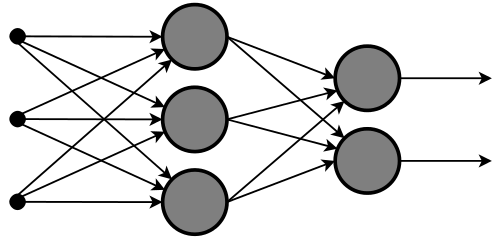
\includegraphics[width=100mm]{img/neural_network.png}
    \caption{An illustration of a multi-layer artificial neural network. }
    \source{Offnfopt / CC-BY-SA 3.0.}
    \label{fig:mlf}
  \end{center}
\end{figure}

\subsection{Structure}
Artificial neural networks can be constructed in different ways, but the most common is the so called \textit{multi-layer feed-forward neural network}, illustrated in Figure~\ref{fig:mlf}. It consists of neurons ordered into multiple layers, the first layer being the \textit{input layer} and the last one the \textit{output layer}. The layers in between are called \textit{hidden layers}. Each neuron is connected with all the neurons in the next layer, with every connection from neuron $i$ to neuron $j$ having a weight coefficient $w_{ij}$. In addition, every neuron has a threshold coefficient, or bias $b_i$. Using these coefficients and all the inputs from the previous layer, every neuron produces an output $x_i$, which can be formally written as follows:
\[x_i = \mathlarger{\varphi}\left(\sum_{j \in \Gamma^{-1}(i)}{w_{ij} \cdot x_j}\right)\]

Here $\Gamma^{-1}(i)$ is notation for the set of all neurons in the previous layer, and $\varphi$ is some \textit{activation function} which squeezes the weighted sum of all input neurons into the range $[0, 1]$, in preparation of passing the output along to the next neuron~\cite{mlfIntro}.

\subsection{Activation functions}
There are many possible choices for the activation function, but three of the most common ones can be found in Table~\ref{tab:activation_functions}. The softmax activation function is different from the others since it does not work on only one neuron, but instead on all neurons in the layer. In doing this, the softmax function can ensure that the sum of all the output values are equal to $1$, which is a desirable thing for the output layer when classifying into $K$ different classes. This also allows the use the \textit{cross-entropy error function} (see later section), which seems to give higher accuracy than using the sigmoid function and the \textit{least squares error function}~\cite{dunne1997pairing}.

\begin{table}[h]
  \renewcommand{\arraystretch}{1.2}
  \begin{center}
    \caption{Selection of common activation functions.}
    \label{tab:activation_functions}
    \begin{tabular}{cc}
      \textbf{Name} & \textbf{Function} $\varphi(x)$\\
      \toprule
      Sigmoid & $\displaystyle \frac{1}{1 + e^{-x}} $ \\[4mm]
      Rectifier & $\displaystyle \max(0, x)$ \\[3mm]
      Softmax & $\displaystyle \frac{e^{x_i}}{\sum_j^K{e^{x_j}}}$ \\
    \end{tabular}
  \end{center}
\end{table}

\subsection{Error functions}
To be able to train our network, we need some way to determine how `bad' a certain output is. This is done using an \textit{error function}, or \textit{loss function}. This function is averaged on the network's output on all training samples. In a classification task, the averaged loss being low means that the network is good at predicting the correct class given a certain input data. If the network performs perfectly, the error function is generally $0$. \textit{Least squares error} is a traditional error function, and if you let $x$ and $\hat{x}$ be the network's output and the wanted output respectively, the least squares error is defined as~\cite{mlfIntro}

\[ E = \sum_i{\frac{1}{2}(x_i - \hat{x}_i)^2} \] 

There is however also another error function that was mentioned earlier, the \textit{cross-entropy error} function. This has some theoretical advantages over least squares error, such as better handling when the probabilities estimated by the network is small, as well as being less dominated by large outliers. Experiments also suggest that these advantages are large enough to be useful in practice. The cross-entropy is defined as~\cite{crossentropy_squared}

\[ E = \sum_i{\hat{x}_i\left(\frac{x_i}{\hat{x}_i}\right)} \]

\newpage
\subsection{Gradient descent}
\begin{wrapfigure}{r}{0.3\linewidth}
  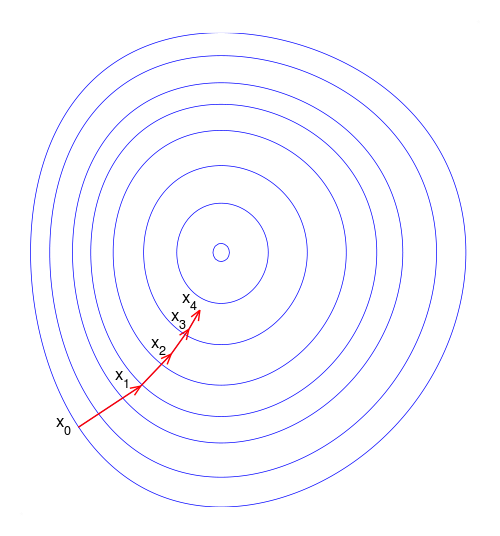
\includegraphics[width=1.6\linewidth]{img/gradient_descent.png}
  \caption{Illustration of gradient descent.}
  \label{fig:gradient_descent}
\end{wrapfigure}
To train a neural network, we want to change the weights and biases (the network's parameters) such that the error on the training set becomes as low as possible. This is done using a process called \textit{gradient descent}. Given the error function and the dataset, the neural network can be viewed a giant function, taking all the parameters as input. By finding the slope or \textit{gradient} of the parameters in the direction that decreases the error, the parameters can gradually be adjusted to find a minimum of the error function. This process is illustrated in Figure~\ref{fig:gradient_descent}. Since this gradient is calculated using the entire dataset to perform a single step, it is known as \textit{batch} gradient descent. Due to this batch gradient descent can become very slow on large datasets, and does not work at all if the dataset does not fit in memory~\cite{gradient_descent}

Because of this a variant of gradient descent named \textit{stochastic} gradient descent (SGD) is sometimes used, where the gradient is calculated using only a single training example at a time. This makes updates to the parameters much faster, but also causes the error function to jump around. This fluctuation adds noise, but also helps the model to not get stuck in local minima. SGD also has the benefit of allowing online learning, where the network can train on new data as it becomes available. In addition the overhead of calculating the gradient this many times might have a negative influence on the final performance~\cite{gradient_descent}.

There is also a third option, \textit{mini-batch} gradient descent, which aims to combine the best of both batch and stochastic gradient descent. Here the gradient calculation is performed on \textit{mini-batches} of $n$ training examples. This can help by making the updates more stable, and also helps with utilizing optimized matrix libraries that enables quickly calculating the gradient for a mini-batch. This is the method typically used when training neural networks in practice, and the term SGD is usually used to refer to this method as well~\cite{gradient_descent}.

\subsubsection{Adam optimizer}
\textit{Adam} is another, more recent method for gradient-based optimization. Its hyperparameters (parameters that adjust how the optimization method works) are intuitive and require little tuning, at the same time as Adam has high efficiency. It compares favorably to other optimization methods, and is well-suited for use in machine learning problems~\cite{adam}.

\subsection{Learning rate}
The learning rate is a parameter that determines how large steps should be taken when performing the gradient descent. Too large a learning rate, and the network will not converge. Too small, and the convergence will take too long. A common strategy is to keep decreasing the learning rate as training progresses~\cite{Bottou2012}.

\section{Convolutional neural networks}

\subsection{Motivation}
One of the largest limitations of traditional artificial neural networks is that they struggle with the complexity of images. The input of a grayscale image of just $112 \times 112$ pixels require \num{12544} connections for every neuron in the first hidden layer. This means that the network has to have a very large number of parameters, which results in training of the network becoming very computationally demanding, as well as increasing the chances of overfitting. A model with fewer parameters to train makes overfitting less likely, which improves the network's performance~\cite{cnnIntro}.

\subsection{Structure}
Convolutional neural networks (CNNs) are specifically designed to work with images as input, and therefore has a different structure than traditional neural networks.
The neurons in a layer are not connected to the all neurons in the preceding layer, instead only connecting to a small region of it.
CNNs have three different types of layers: \textit{convolutional} layers, \textit{pooling} layers, and \textit{fully-connected} layers.
The layers are said to have three dimensions: height, width, and depth. The initial height and width correspond to the input image dimensions, while the depth represents different \textit{feature maps}.
If the images the network trains on are grayscale and has size $112 \times 112$, the input `volume' will have the dimension $(112, 112, 3)$~\cite{cnnIntro}.

\subsection{Convolutional layers}
Convolutional layers consists of a number of different \textit{filters}. These filters usually have small dimensions, say $(3, 3)$, but works on the entire depth of the input and are used to sweep, or \textit{convolve}, over the input's width and height. A $3 \times 3$ filter would have $3 \times 3 \times depth$ adjustable parameters, which forms the filter's \textit{kernel}. The output value, which will be located at the pixel in the center of the filter, is the dot product of the kernel and the current input region~\cite{cnnIntro}. For an illustration of this see Figure~\ref{fig:cnn_color_filter}.

\begin{figure}
  \begin{center}
    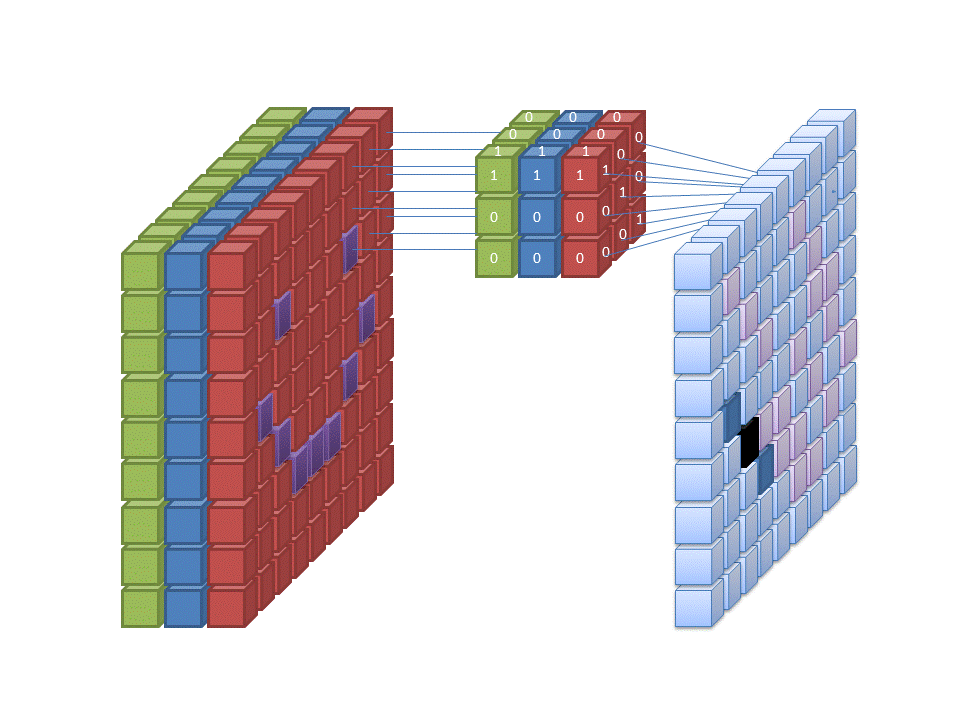
\includegraphics[width=100mm]{img/cnn_color_filter.png}
    \caption{Illustration of a filter on a color image.}
    \source{Cecbur / CC-BY-SA 4.0.}
    \label{fig:cnn_color_filter}
  \end{center}
\end{figure}

The depth of a layer's output volume in the CNN can be increased by increasing the number of filters used. The filters can pick up on different features, of which the intensity in different regions of the image will be outputted in the different depth dimensions, and picked up by later layers.

Another parameter that can be adjusted for the layer is the \textit{stride}. A stride of $1$ means that the filter is moved one step at a a time, while a higher stride of $n$ can be used to make the filter only evaluate every $n^{\text{th}}$ possible position. This reduces overlap, but has the benefit of shrinking the output volume.

For filters of size larger than $1 \times 1$, the output will have slightly smaller dimensions since the filter can't go outside the edge of the input. To avoid missing features on the edges, \textit{zero-padding} is often used. This pads the input volume with enough zeroes to make the output volume the correct size, enabling the filter to be positioned right on the edge~\cite{cnnIntro}.

\subsection{Pooling layers}
A different way of shrinking the layers' spatial dimension are \textit{pooling layers}. These are used to gradually reduce the representation's dimensionality, which reduces the total amount of parameters that need to be trained. The most common method is by using $2\times 2$ max-pooling layer. This is applied with stride 2 on the input volume, shrinking the output width and height by 2 and reducing the total output size to 25~\%. As the name implies, the output of the filter is the maximum of the input values in the region as shown in Figure~\ref{fig:max_pooling}. Pooling retains the number of depth dimensions~\cite{cnnIntro}.

\begin{figure}
  \begin{center}
    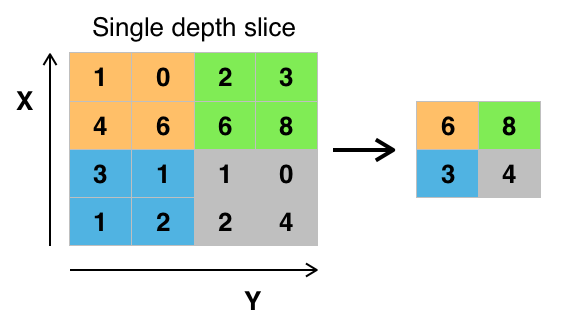
\includegraphics[width=80mm]{img/max_pooling.png}
    \caption{Example of max pooling.}
    \source{Aphex34 / CC-BY-SA 4.0.}
    \label{fig:max_pooling}
  \end{center}
\end{figure}

\subsection{Fully-connected layers}
The fully connected layers work just like they do in traditional neural networks, and are often placed at the end of a CNN network. This lets them compact all the data in the final volume into the final output of the network.

\subsection{Common architectures}
Commonly a CNN is constructed by stacking pairs of convolutional and pooling layers, before finally ending with fully-connected layers. This convolutional outputs are passed through the rectifier activation function. Another common option is to have two convolution layers before the pooling layers. This is recommended since it allows the network to learn more complicated features. The general trend in the layer volume dimensions is that they become smaller but deeper towards the end of the network~\cite{cnnIntro}. For an illustration of a typical complete CNN architecture, see Figure~\ref{fig:typical_cnn}.

\begin{figure}
  \begin{center}
    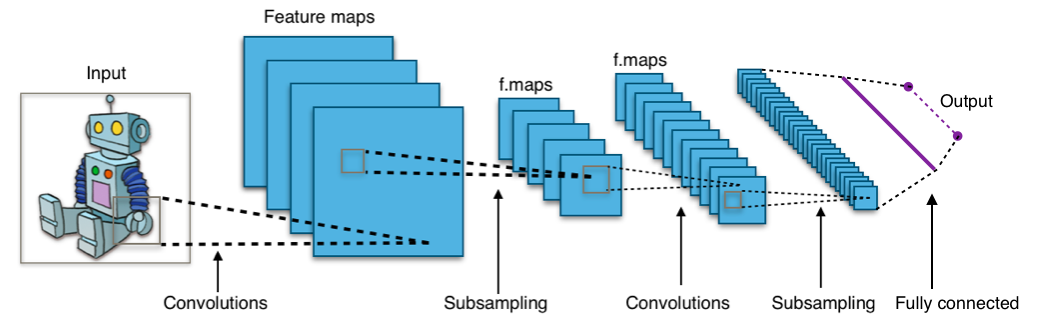
\includegraphics[width=150mm]{img/typical_cnn.png}
    \caption{Illustration of a typical CNN architecture.}
    \source{Aphex34 / CC-BY-SA 4.0.}
    \label{fig:typical_cnn}
  \end{center}
\end{figure}

\section{Evaluation of classification systems}
To evaluate a classification system an objective scoring method is needed. The most common method uses the two values \textit{precision} and \textit{recall}, together with the combined measure \textit{F1-score}. These can be calculated from the the number of true positives (TP), true negatives (TN), false positives (FP), and false negatives (FN). Descriptions of these can be found in Table~\ref{tab:tp_mm}. Precision and recall correspond to the medical terms \textit{specificity} and \textit{sensitivity}, respectively. Using these measures instead of the accuracy (the ratio of correct classifications) provides more information about what kinds of mistakes a model makes.

\begin{table}[H]
  \begin{center}
    \begin{tabular}{cc}
      \textbf{Name} & \textbf{Meaning} \\
      \toprule
      TP & Hits, number of correct identifications. \\
      TN & Number of correct rejections. \\
      FP & False alarms, number of incorrect identifications. \\
      FN & Misses, number of incorrect rejections.
    \end{tabular}
  \end{center}
  \caption{Explanation of classification results.}
  \label{tab:tp_mm}
\end{table}

\subsubsection{Precision}
In the context of classification, the fraction of guesses on a certain class that is correct is said to be the \textit{precision} of the model on this class~\cite[p.~5]{irbook}.
\[ P = \frac{\text{TP}}{\text{TP} + \text{FP}} \]

\subsubsection{Recall}
In the context of classification, the fraction of instances of class which are correctly identified is said to be the \textit{accuracy} of the model on this class~\cite[p.~5]{irbook}. This is also known as \textit{sensitivity}.
\[ R = \frac{\text{TP}}{\text{TP} + \text{FN}} \]

\subsubsection{F1-Score}
The F1-score can be used to combine the precision and recall scores into a single measure. It is defined to be the harmonic mean of precision and recall~\cite[p.~156-167]{irbook}, which can be written as
\[ F_1 = \frac{2PR}{P + R} \]

\section{Previous work}
Studies focusing specifically on the effect of different training methods on neural networks, convolutional or otherwise, seems to be rare. This is especially true for the smaller subject of machine learning on medical images.
What do exist, however, is \textit{guidelines} for how you should train networks in various scenarios, as well as studies where researches create and evaluate a specific CNN model. Three studies will be highlighted here: One for the case of medical images, one for the handling of imbalanced dataset, and finally one study which achieves high performance on classification of Alzheimer's disease.

\subsection{Training CNNs on medical images}
In the book \citetitle{deepmedical}, suggestions for how to train machine learning models in the context of medical images are described. They suggest three general methods for improving learning: The use of rectified linear units (ReLU), dropout, and batch normalization~\cite[p. 20-22]{deepmedical} These will not be evaluated in this study, however ReLU units will be used in the CNN (see Section~\ref{methods}).
In addition, \citetitle{deepmedical} highlights the usefulness of data augmentaion, where geometric transforms are applied to the training data in order to extend it. This is said to typically increase performance by about 3~\%~\cite[p. 31]{deepmedical}.

\subsection{Handling imbalanced datasets}
Training of machine learning models for classification problems often suffers from imbalance in the dataset between the different classes. This is studied in \citetitle{more2016survey}, by \textcite{more2016survey}.

Three general solutions, along with more or less complicated variants, were evaluated on a synthetic imblanaced dataset. The goal is to improve recall on the rare class, while not worsening the precision of the common class. First of the methods are \textit{class-weighting}, where the error function is modified to weigh each class equally, disregarding the relative sizes. Second is \textit{undersampling}, where samples of the common class are skipped when training. Finally there is \textit{oversampling}, where the rare class is made larger. On their dataset, a variant of oversampling called \textit{SMOTE} in combination with class-weighting was found to be the most effective. Granted that, the article also notes that the most effective method may vary depending on the data distribution~\cite{more2016survey}.

\subsection{Classification of Alzheimer's disease}
Many studies exist describing systems classifying MRI images as either having Alzheimer's disease or not. Many different methods have been used, including linear support vector machines by \textcite{cuingnet2011automatic}, deep CNNs by \textcite{sarraf070441}, probability distribution functions by \textcite{beheshti2015probability}, as well as strateges combining MRI with multiple biomarkers and machine learning models such as the one by \textcite{zhang2011multimodal}.

\subsubsection{Multi-class classification}
\textcite{islam2018early} studied a variation of Alzheimer's disease classification, where classification is done into four different classes (based on CDR scores), instead of just two. Their method was a variant of a CNN that they trained on the OASIS dataset~\cite{oasis}. Their CNN uses uses a densely connected architecture that seems identical to DenseNet~\cite{huang2017densely}. While their model showed acceptable performance for identifying non-demented patients, its performance on classifying demented patients was significantly worse, which they speculate could be because of the limited number of samples~\cite{islam2018early} in OASIS\@. Their performance can be viewed in Table~\ref{tab:results_islam_zhang}.

\begin{table}
  \begin{center}
    \caption{Results by \textcite{islam2018early}. \label{tab:results_islam_zhang}}
    \begin{tabular}{r|ccc|c}
      \textbf{CDR Class} & \textbf{Precision} & \textbf{Recall} & \textbf{f1-Score} & \textbf{Support} \\
      \toprule
      Non-demented (0.0) & 0.99 & 0.99 & 0.99 & 73 \\
      Very mild (0.5) & 0.75 & 0.50 & 0.60 & 6  \\
      Mild (1.0)         & 0.62 & 0.71 & 0.67 & 7  \\
      Moderate (2.0)     & 0.33 & 0.50 & 0.40 & 2   \\
    \end{tabular}
  \end{center}
\end{table}

\chapter{Methods} \label{methods}
This report will evaluate two different strategies for training a convolutional neural network, comparing them to a baseline. The structure of the CNN used is described in Section~\ref{network_structure}. This CNN was trained and evaluated using the OASIS-3 dataset, presented in Section~\ref{dataset}. The training methods examined were:
\begin{enumerate}
  \item Baseline
  \item Training with equal weighting of the different classes (\textit{class-weighting})
  \item Training utilizing \textit{data augmentation}
\end{enumerate}

The network was trained for \num{1000} epochs (one epoch is one run through all training data) for the \textit{Default} and \textit{class-weighted} training regimes. The last training method using data augmentation was allowed to run for \num{5000} epochs, since convergence was much slower. The accuracy on the different classes were measured for each method. Most similar studies report their performance using precision, recall, and f1 score. The same performance metrics will be used in this study, both for their inherent usefulness and to make comparisons possible.

\section{Training methods}
\subsection{Baseline}
\textit{Baseline training} is the least sophisticated method, and is what would be used by someone who does not put any thought into how the training should work. This is what popular machine learning frameworks will provide by default, and will provide a performance baseline. The other two methods are meant to counter the problems the baseline training strategy might have in our use case.

\subsection{Class-weighting}
Like the original OASIS, OASIS-3 contains many times more images of patients without or with mild Alzheimer's disease as with more severe cases (see Section~\ref{dataset}). In the study by~\textcite{islam2017novel}, they tried to correct this by weighing each class equally in the error function, no matter how large part of the dataset each class actually represents. This will be the second training method tested, to see if data augmentation solves the issue of an imbalanced dataset and improves the performance on the rarer classes.

\subsection{Data augmentation}
When the size of the dataset is not too large, there is a risk of overfitting. Overfitting is when the network `memorizes' the data used in the training set. This causes it to have very high performance and low error on the training data, while not being able to perform well in general which will be visible when testing on the validation data. One way to battle this is data augmentation, where the dataset is in some way extended. For this test the images will be mirrored along the sagittal axis (right side of the brain will become the left), as well as zoomed in or out a random amount at most 20~\%. This will, in effect, produce an infinite training dataset (albeit a quite homogenous one). This larger dataset will in theory make overfitting less likely. However, this will not change the proportion of the training classes. When training, an image is selected from the original dataset. This image is then used to create an augmented image, keeping which keeps the class ratio the same.

\section{OASIS-3 dataset} \label{dataset}
OASIS-3 is a longitudinal neuroimaging dataset, with data collected over the course of 30 years from 1098 adult participants from multiple studies. Of these participants 809 were cognitively normal, while 489 were at various stages of cognitive decline. Accompanying the neural imaging is (among other things) clinical assessments of cognitive function~\cite{oasis3}. I will use the T1-weighted brain scans and mental assessments which were done using the CDR system. The dataset in total contains 3393 T1-weighted MRI images and 4089 different CDR evaluations.

The subset of the dataset that was used contains 2782 images (see skipped images in Section~\ref{image_extraction}). Of these images 20~\% were selected to be used as validation data, while the other 80~\% was used to train the network. Since the network has never seen the validation data during training, it can be used to evaluate its expected performance on unknown MRI images. Just as in the paper by \textcite{islam2018early}, the CDR scores were used to divide the images into four classes: \textit{non-demented}, \textit{very mild dementia}, \textit{mild dementia}, and \textit{moderate dementia}. These classes are not equally represented in the dataset, with the more serious dementia cases being much less frequent. The total count of each class is shown in Table~\ref{tab:dataset_contents}, together with the image count in the training and verification sets.

\begin{table}[h]
  \begin{center}
    \caption{Count of images belonging to each class in the dataset.\label{tab:dataset_contents}}
    \begin{tabular}{r|cccc}
      \textbf{CDR Class} & \textbf{Total} & \textbf{Training set} & \textbf{Validation set} \\
      \toprule
      Non-demented (0.0) & 2162 & 1722 & 440 \\
      Very mild (0.5) & 442 & 362 & 80 \\
      Mild (1.0) & 152 & 121 & 31 \\
      Moderate (2.0) & 22 & 17 & 5 \\
      \bottomrule
      \textbf{Sum} & 2778 & 2222 & 556 \\
    \end{tabular}
  \end{center}
\end{table}

\section{Labeling}
The assessment of the subjects' CDR score was used to label every MRI image with the stage of dementia. However, since OASIS-3 is a longitudinal study, the MRI scans and the clinical assessments were not performed at the same time. In fact, the time between MRI scans and the closest CDR assessment can be relatively large ($\mu=116$, $\sigma=107$). The distribution is shown in Figure~\ref{fig:mri_cdr_offset}. For most of the data the time from an MRI scan to the closest CDR assessment is less than 200 days, while for some images the delay can be several hundred days.

To try to get reasonable CDR labels even when the time differences are large, a linear interpolation of the two closest CDR assessments considering the time of the MRI scan was used when this was possible. If the MRI scan was done either before or after all of this subject's CDR assessments, the MRI scan was tagged with the closest CDR value.

This CDR calculation can be written as follows:
\begin{flalign*}
  \begin{aligned}
    \text{cdr} &=
    \begin{cases}
      \text{cdr}_{\text{next}} & \text{if before all assessments} \\
      \text{cdr}_{\text{prev}} & \text{if after all assessments} \\
      \text{cdr}_{\text{prev}} + x * (\text{cdr}_{\text{next}} - \text{cdr}_{\text{prev}}) & \text{otherwise} \\
    \end{cases} & \\[5pt]
    \text{where }x &= \frac{\text{day}_{\text{MRI}} - \text{day}_\text{prev}}{\text{day}_{\text{prev}} - \text{day}_{\text{next}}}&
  \end{aligned}
\end{flalign*}

Here $0 \leq x \leq 1$ is the interpolation factor between the two assessments closest to $\text{day}_{\text{MRI}}$, the day the MRI scan was done.

\begin{figure}
  \begin{center}
    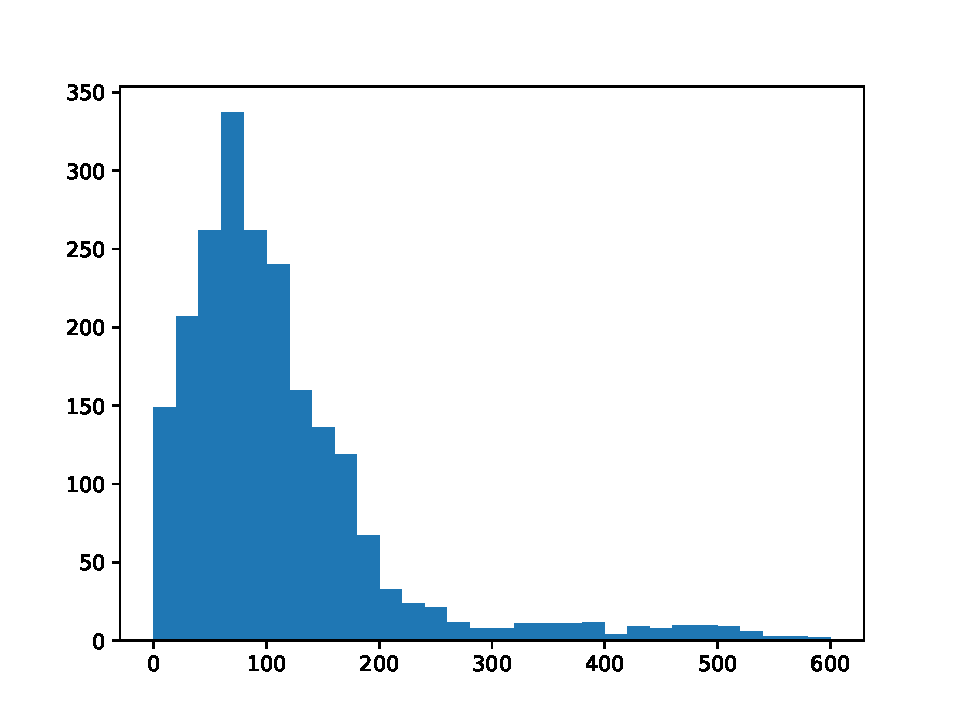
\includegraphics[width=100mm]{img/mri_cdr_offset.pdf}
    \caption{Histogram of time between MRI scans and the closest CDR assessment (in days).}
    \label{fig:mri_cdr_offset}
  \end{center}
\end{figure}



\begin{minipage}{.7\linewidth}
\vspace*{-50mm}
\section{Image extraction} \label{image_extraction}
During the preprocessing step the image plane were extracted from each MRI scan. For simplicity the planes chosen are the middle one for each axis, and the raw intensity values from each scan are flattened into the normal black/white range of PNG images.

Some MRI scans are rotated the wrong way, even after trying to orient them correctly using the metadata from the scan. These images are not corrected but instead skipped.

\section{Hyperparameters}
As mentioned earlier the Adam optimizer was used. It was instantiated with a learning rate of $10^{-5}$, a beta$_1$ of $0.9$, a beta$_2$ of $0.999$, an epsilon of $10^{-7}$, and no weight decay. When training a batch size of $64$ was used.

Whn choosing hyperparameters, the learning rate of the Adam optimizer was found to be important. The default learning rate of $0.001$ appears to be to large, and results in the network not improving. A lower rate of $10^{-5}$ resulted in better and quicker results during training.

\section{Network structure} \label{network_structure}
The network this study is going to evaluate is mostly based on the basic CNN design suggested by \textcite{cnnIntro}, with double convolutional layers joined by pooling layers. The first two layers are taken from \textcite{islam2018early}, and consists of a convolutional layer with filters of size $7 \times 7$ and stride 2, followed by a pooling layer. The sequence of layers can be seen in Figure~\ref{fig:network_structure}. All the other convolutional layers use filters of size $3 \times 3$. At the end of the network there are 128 fully connected neurons which finally connect into the four output neurons. Each output neuron represents the probability of each class. The densely connected layer also uses rectified linear activation, while the output layer uses softmax activation. The network is trained using the Adam optimizer, which is a variant of SGD, and the cross-entropy loss function.

\end{minipage}
\begin{minipage}{.3\linewidth}
  \centering
  \vspace*{-20mm}
  \hspace*{0mm}
  \begin{figure}[H]
      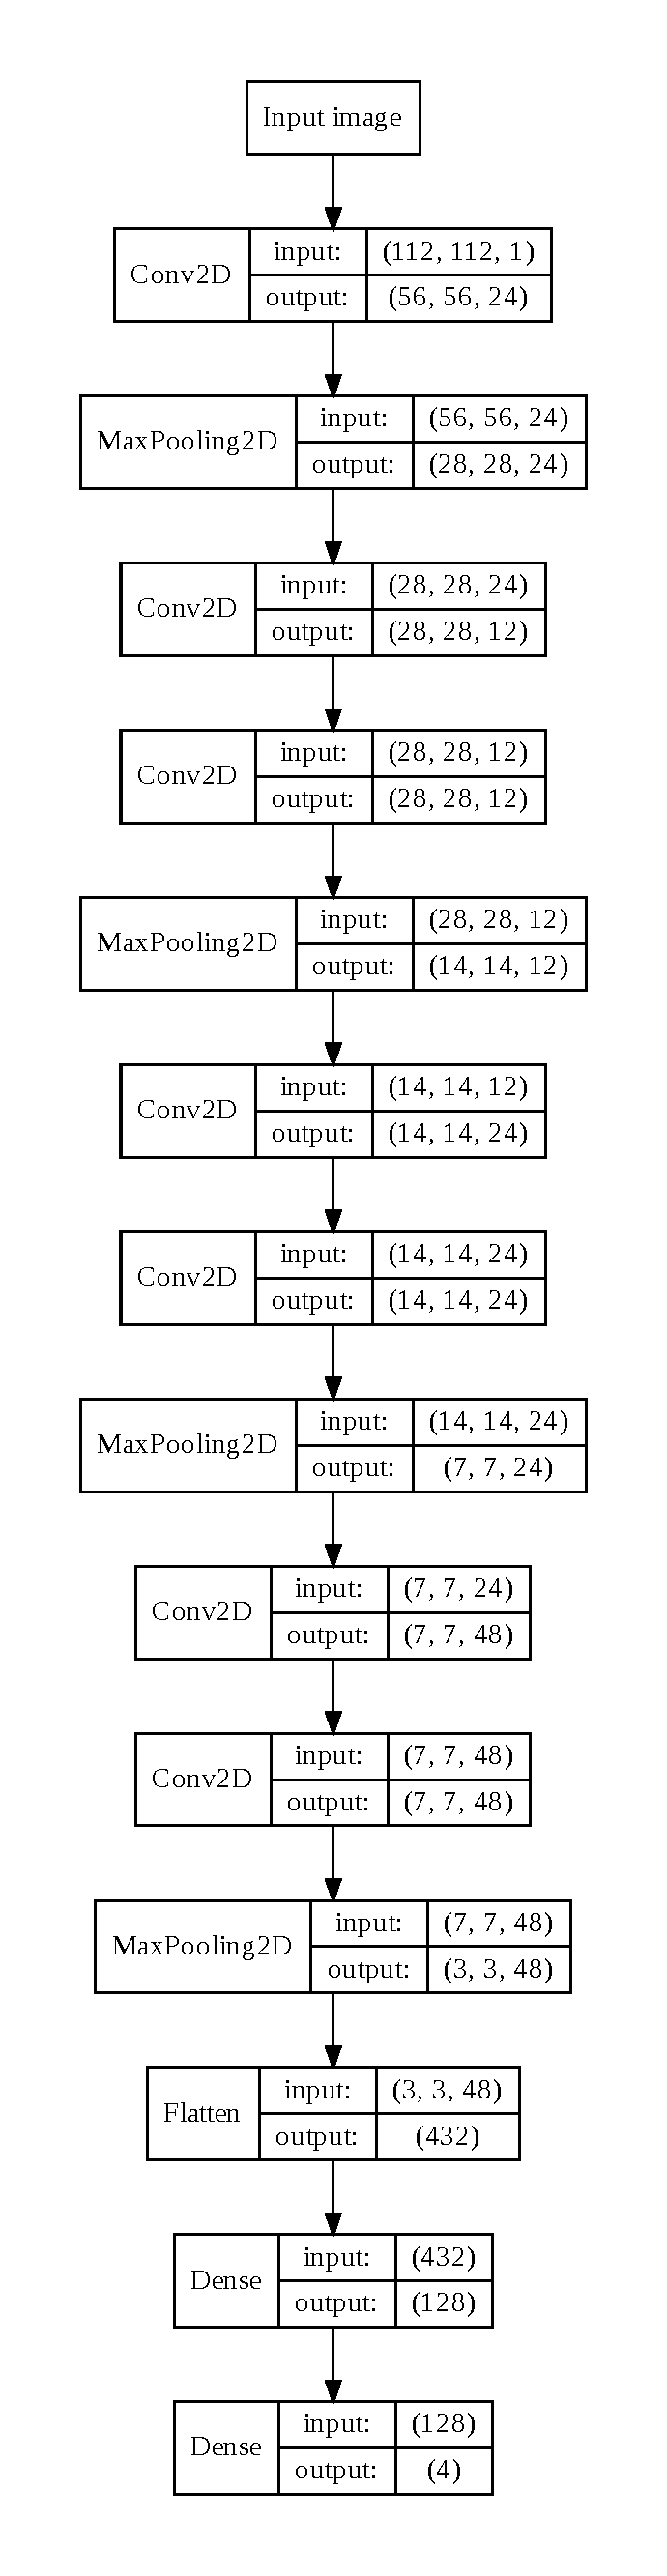
\includegraphics[width=1.7\textwidth]{img/model.pdf}
      \vspace*{-13mm}
      \caption{Diagram of the CNN used in this study.}
      \label{fig:network_structure}
  \end{figure}
\end{minipage}

\chapter{Results}

For each of the two methods, in addition to the default baseline, the results will be presented as one table, and two diagrams. The table presents the precision, recall, and f1-score for each method on each class. The support column of the table shows the number of datapoints in each class.Then follows the two diagrams. The first shows the evolution of the loss function for both test and validation data during the training, on a logarithmic scale, while the other shows the evolution of the accuracy.

\section{Baseline}
\begin{table}[H]
  \begin{center}
    \caption{Baseline results. \label{tab:results_default}}
    \begin{tabular}{r|ccc|c}
      \textbf{CDR Class} & \textbf{Precision} & \textbf{Recall} & \textbf{f1-Score} & \textbf{Support} \\
      \toprule
      Non-demented (0.0) & 0.88 & 0.91 & 0.89 & 440 \\
      Very mild (0.5) & 0.51 & 0.46 & 0.49 & 80  \\
      Mild (1.0)         & 0.40 & 0.32 & 0.36 & 31  \\
      Moderate (2.0)     & 0.33 & 0.20 & 0.25 & 5   \\
    \end{tabular}
  \end{center}
\end{table}

As can be seen in Table~\ref{tab:results_default}, the network achieves high performance on the \textit{Non-demented} class (f1-score of 0.89), but as the classes get rarer performance deteriorates. Especially bad is the recall, with a value of just $0.20$ on the \textit{Moderate} class.

The validation loss, presented in Figure~\ref{fig:loss_default}, can be seen to quickly decrease together with the training loss, and then slowly start increasing while the training loss decreases. For the accuracy presented in Figure~\ref{fig:accuracy_default}, note the `bump' in accuracy at the beginning, and the following gap as test accuracy rises to $1$ while validation accuracy stays around $0.80$.

\begin{figure}[H]
  \centering
  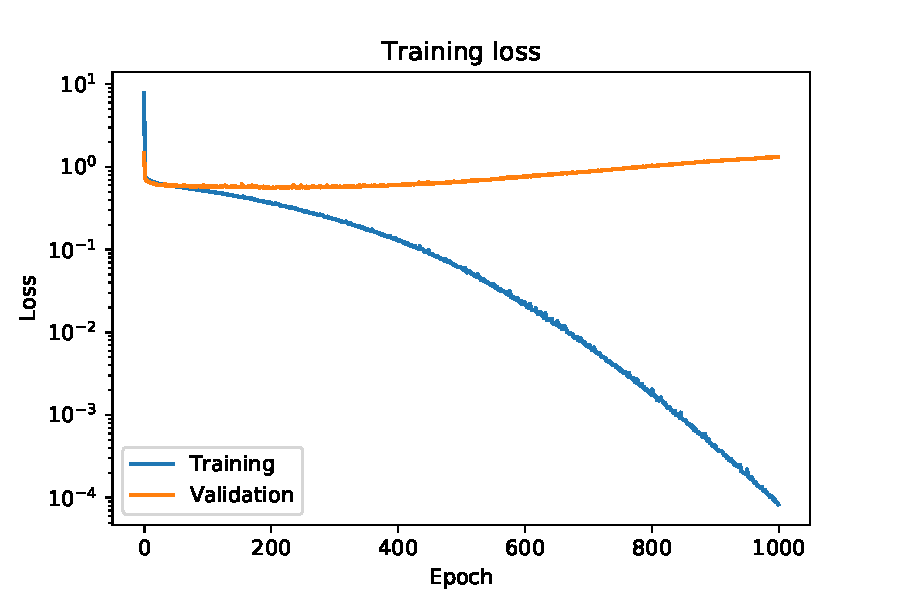
\includegraphics[width=0.9\linewidth]{img/loss_default.pdf}
  \caption{Loss during training with the baseline training scheme.} \label{fig:loss_default}
\end{figure}
\begin{figure}[H]
  \vspace{-3mm}
  \centering
  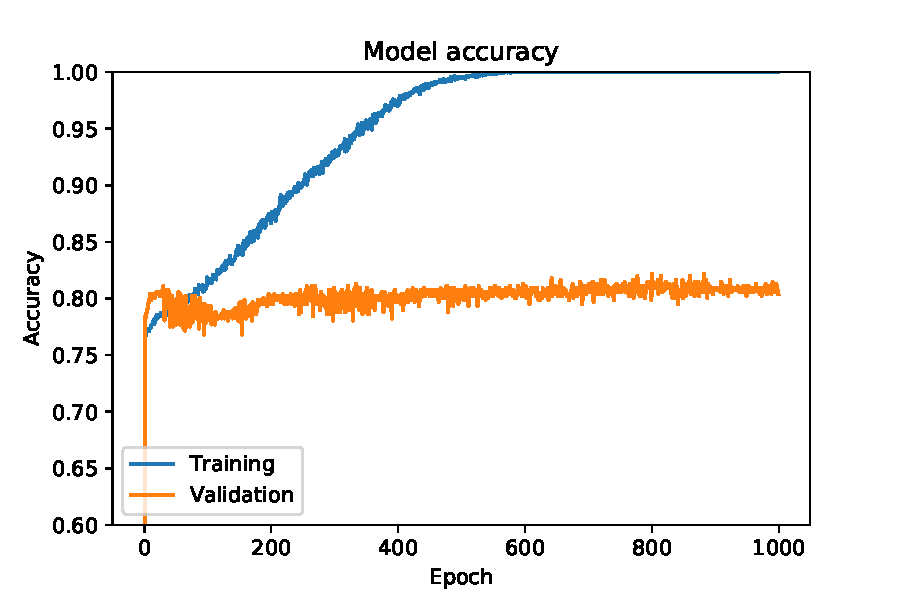
\includegraphics[width=0.9\linewidth]{img/accuracy_default.pdf}
  \caption{Accuracy during training with the baseline training scheme.} \label{fig:accuracy_default}
\end{figure}


\section{Class-weighted training}
\begin{table}[H]
  \begin{center}
    \caption{Results for class-weighted training. \label{tab:results_class_weighted}}
    \begin{tabular}{r|ccc|c}
      \textbf{CDR Class} & \textbf{Precision} & \textbf{Recall} & \textbf{f1-Score} & \textbf{Support} \\
      \toprule
      Non-demented (0.0) & 0.87 & 0.93 & 0.90 & 440 \\
      Very mild (0.5) & 0.52 & 0.41 & 0.46 & 80  \\
      Mild (1.0)         & 0.43 & 0.29 & 0.35 & 31  \\
      Moderate (2.0)     & 1.00 & 0.60 & 0.75 & 5   \\
    \end{tabular}
  \end{center}
\end{table}

As can be seen in Table~\ref{tab:results_class_weighted}, the networks achieves high performance on the \textit{Non-demented} class (f1-score of 0.9). The model does not perform as well on the \textit{Very mild} class (f1-score of 0.46), and even worse on the \textit{Mild} class (f1-score of 0.32). Nevertheless, note the high performance of the \textit{Moderate} class (precision of $1.0$ and recall of $0.60$).

The training and validation loss has a large gap, as can be seen in Figure~\ref{fig:loss_class_weighting}. The accuracy shown in Figure~\ref{fig:accuracy_class_weighting} starts out low, below the bottom of the diagram at $0.60$, but then increases. Training accuracy increases faster towards $1.0$, while validation accuracy more slowly plateaus at $0.80$.
\newpage

\begin{figure}[H]
  \centering
  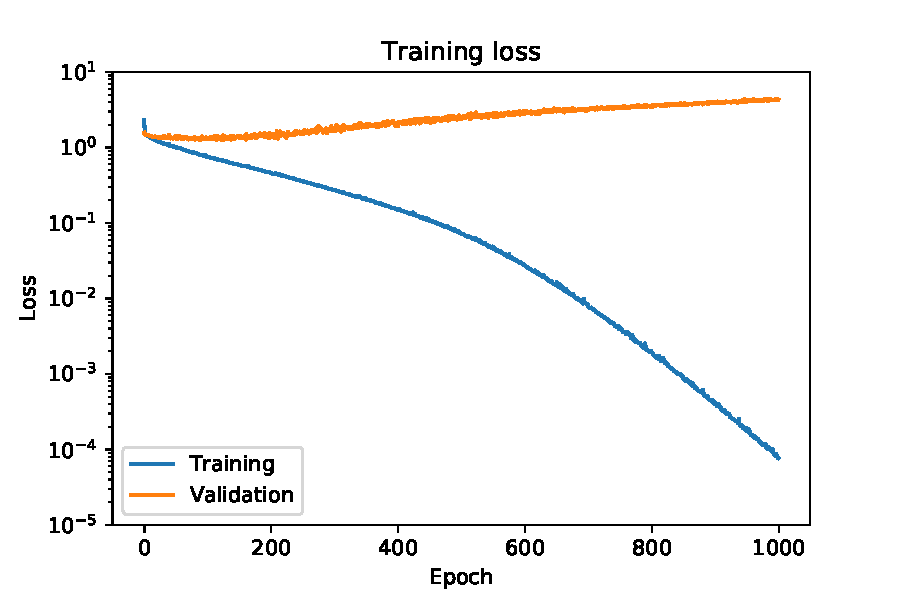
\includegraphics[width=0.9\linewidth]{img/loss_class_weighted.pdf}
  \caption{Loss during training with class-weighting.} \label{fig:loss_class_weighting}
\end{figure}
\begin{figure}[H]
  \centering
  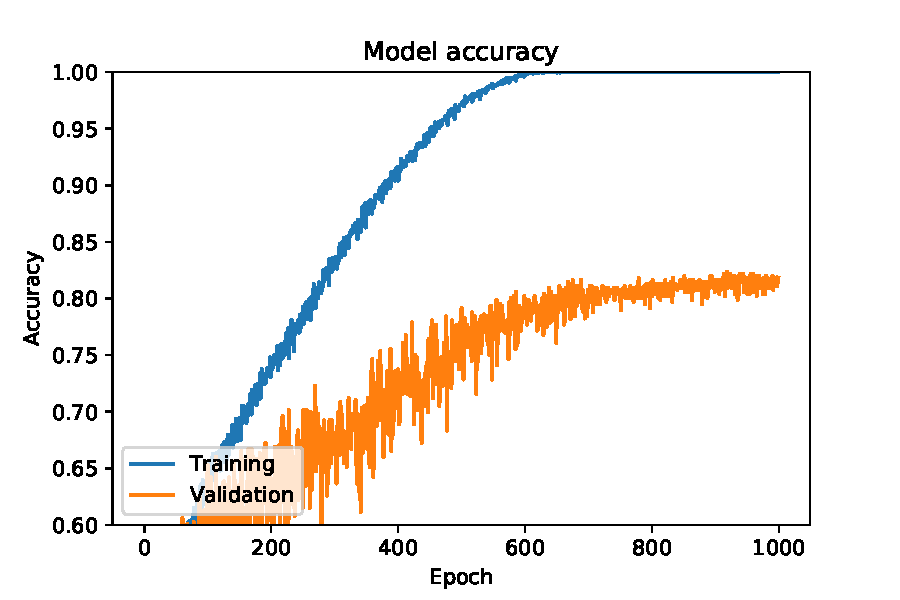
\includegraphics[width=0.9\linewidth]{img/accuracy_class_weighted.pdf}
  \caption{Accuracy during training with class-weighting.} \label{fig:accuracy_class_weighting}
\end{figure}

\section{Training with data augmentation}

\begin{table}[H]
  \begin{center}
    \caption{Results with data augmentation. \label{tab:results_data_augmentation}}
    \begin{tabular}{r|ccc|c}
      \textbf{CDR Class} & \textbf{Precision} & \textbf{Recall} & \textbf{f1-Score} & \textbf{Support} \\
      \toprule
           Non-demented (0.0) &  0.91   &  0.77  &   0.83   &   440 \\
           Very mild (0.5) &  0.33   &  0.57  &   0.42   &    80 \\
           Mild (1.0)         &  0.40   &  0.55  &   0.46   &    31 \\
           Moderate (2.0)     &  0.67   &  0.40  &   0.50   &     5 \\
    \end{tabular}
  \end{center}
\end{table}

Looking at Table~\ref{tab:results_data_augmentation}, \textit{Non-demented} precision is high (0.91), but recall is lower (0.77). Precision on the \textit{Very mild}, \textit{Mild}, and \textit{Moderate} classes was low ($0.33$, $0.40$, and $0.67$ respectively) with recall being slightly higher ($0.57$, $0.55$, and $0.40$ respectively).

The training and validation loss presented in Figure~\ref{fig:loss_data_augmentation} stick together relatively closly. Note also that the training accuracy in Figure~\ref{fig:accuracy_data_augmentation} does not reach $1.0$, instead following the validation accuracy without departing significantly.
\newpage

\begin{figure}[H]
  \centering
  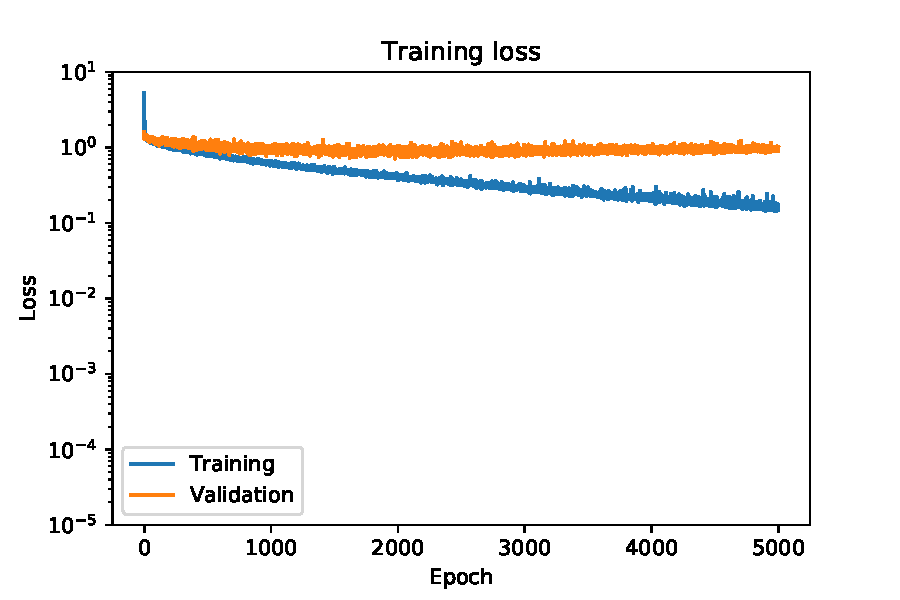
\includegraphics[width=0.9\linewidth]{img/loss_data_augmentation.pdf}
  \caption{Loss during training with data augmentation.} \label{fig:loss_data_augmentation}
\end{figure}
\begin{figure}[H]
  \centering
  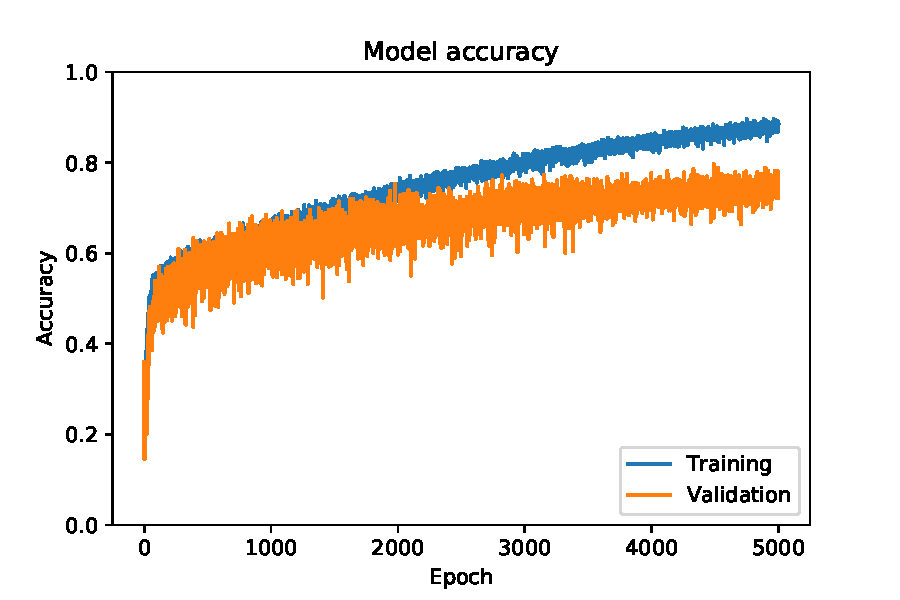
\includegraphics[width=0.9\linewidth]{img/accuracy_data_augmentation.pdf}
  \caption{Accuracy during training with data augmentation.}\label{fig:accuracy_data_augmentation} 
\end{figure}

\section{Summary of training results}
For easy visual comparison, the precision and recall for the three training methods on each class can be found in Figure~\ref{fig:precision_comparison} and Figure~\ref{fig:recall_comparison}, respectively.

Class-weighting is seen to not decrease precision much on any class, while improving the precision significantly on the \textit{Moderate class}. Recall was found to deteriorate slightly on \textit{Very mild} and \textit{Mild} classes, while improving slightly on \textit{Non-demented} and significantly on \textit{Moderate}.

Data augmentation increases precision slightly on the \textit{Non-demented} class, while decreasing precision heavily on the \textit{Very mild} and \textit{Moderate} classes. Recall is decreased on \textit{Non-demented} and \textit{Moderate}, while increasing for the other two classes.
\newpage

\begin{figure}[H]
  \centering
  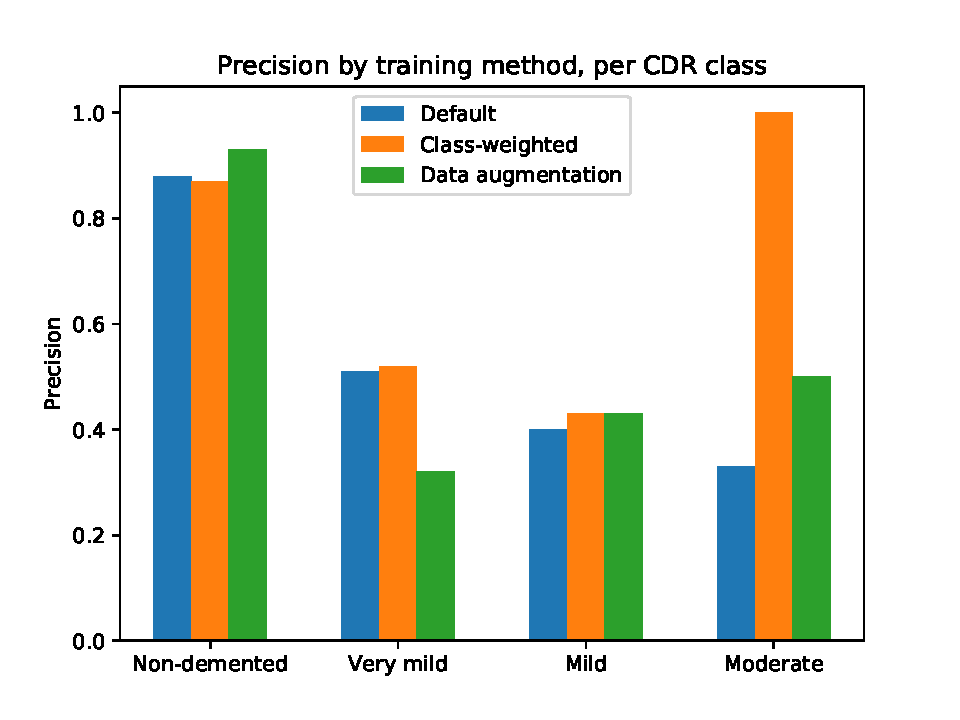
\includegraphics[width=0.8\linewidth]{img/precision_comparison.pdf}
  \caption{Comparison of the precision resulting from the different training methods.} \label{fig:precision_comparison}
\end{figure}
\begin{figure}[H]
  \centering
  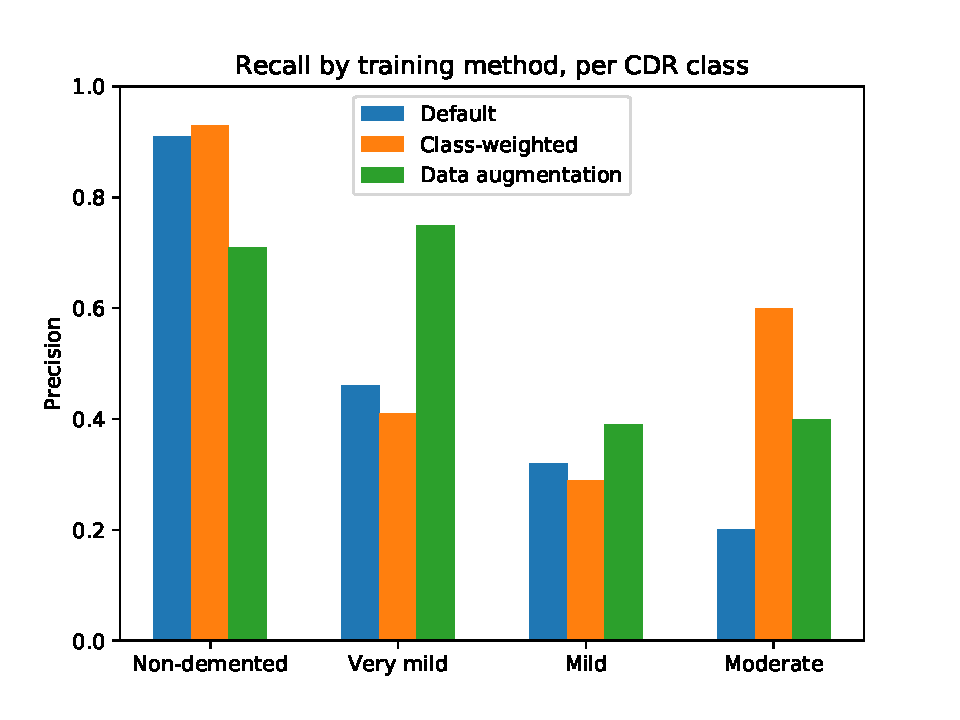
\includegraphics[width=0.8\linewidth]{img/recall_comparison.pdf}
  \caption{Comparison of the recall resulting from the different training methods.} \label{fig:recall_comparison}
\end{figure}

\chapter{Discussion}

\section{Method}
It is debatable exactly what good performance is in the area of computer-aided medical diagnostics. Is it more important that the model does not miss any cases of disease (minimize false negatives), or that the model does cause any false alarms (minimize false positives)? Aditionally, in multi-class classification like the one performed here, are some classes more important than others? This is not obvious, but most likely the model should prioritize finding all cases of disease. If some false positives also occur that is fine, as long as the rate is low enough for the model to be useful. For Alzheimer's diagnosis, the most interesting class is probably \textit{Very mild}. Diagnosis of this class would bring the most benefit to patients, as the disease is still not very apparent and in an early stage.

Just as in the study by \textcite{islam2018early}, the low frequency of samples in the dataset showing progressed dementia is an issue. Thanks to OASIS-3 containing many times the number of MRI images as the original OASIS does, this is not as large of a problem during training, with all classes having a a decent amount of images (maybe besides \textit{Moderate}, which only has 22). The low frequency is however very noticeable during validation, when it results in single-digit counts of the rarest class \textit{Moderate}. This gives very rough knowledge of how accurate the model actually is on this type of data, as a single extra correct classifition increases recall by $0.20$. To combat this it might have been useful to increase the ratio of validation to training data, for more stable results. On the other hand, detecting these progressed cases of dementia might no be very useful in practice, since by then the symptoms will be so pronounced that diagnosis using MRI scanning is not required. In the long term it would be beneficial if new and larger datasets were created, that would both give more training data and enable researchers to evaluate their models' performance with more confidence.

The exact CNN model and hyperparameters used was assumed to not have any effect on the relative performance of the different training methods. However, this is just a guess, and might not be true. One must consider the possibility that other network structures and hyperparameters might benefit more or less from the two training methods.

\section{Results}
\subsection{Baseline training}
When training without weighting the classes differently, the network starts out with an accuracy of just below 80~\%. The training data mostly contains images of cognitively normal brains, at a rate of $\frac{1724}{2162} \approx 79.7~\%$. This suggests that the network quickly learns to classify everything as this class, for a large and quick gain in accuracy which will just as quickly decrease the loss. Inspection of the output reveals that yes, this is actually the case the first few epochs. However, after training some more the network begins to try and also classify the other classes, managing a precision ranging from 30~\% to 50~\% on the three demented classifications. The accuracy steadily decreases as the classes get rarer, most likely because the loss function does not encourage exploration in order to get better on them. Since all input samples are weighted equally in the eyes of the loss function, performance on the ca.\ 20 images showing moderate dementia is worth 100 times less than the performance on the ca.\ \num{2000} images showing no dementia. If getting better on the rare classes means getting slightly worse on the dominating one, improvement is not likely. Overfitting seems to be a large problem, with the network quickly reaching 100~\% accuracy on the training data, with nowhere near as good results on the validation set.

\subsection{Class-weighted training}
Weighting each class equally was very important for the most rare class, \textit{Moderate}. The precision on this group increased from $0.33$ to $1.0$, and the recall from $0.20$ to $0.60$. This happened at the same time as the performance on the other classes remained on a similar, slightly higher level, besides on the \textit{Non-demented} class. These decrease was however very small, and not significant. In conclusion, class-weighting was important for the precision of the very rare class, but not as much for the moderately rare.

The recall was also found to improve significantly on the \textit{Moderate} class, as well as increasing slightly on the \textit{Non-demented} class. Interestingly, recall decreased on the \textit{Very mild} and \textit{Mild} classes, despite increased recall on rare classes being one of the main supposed benefits of class-weighting. Perhaps these classes are not rare enough, with only the \textit{Moderate} class being rare enough to improve, or maybe the method simply doesn't work that well on this dataset. Overfitting is still a problem, with training validation reaching 100~\%.

In general, if the dataset contains any rare classes like the \textit{Moderate} class, making sure to not disfavor them could be very important. These rare classes might be obvious, as they are here, but might also be hidden. For example, if a dataset mostly contains data collected from male subjects, a model could be biased during training and perform less well on female data, and vice versa. In cases like this class-weighted training could be essential for fairness.

\subsection{Training with data augmentation}
The results when using data augmentation need to be compared to the class-weighted results, since the data augmentation was used on top of the class-weighting. At a first glance, the results were to my surprise not very impressive. The network still showed signs of overfitting, albeit not as much, and performance did not consistently improve. This suggests that data augmentation is not a universal solution, and other adjustments should be considered to combat overfitting

Precision improveded slightly on \textit{Non-demented}, but at the same time recall decreased significantly which is not desirable. The performance \textit{Moderate} decreased heavily, with both precision and recall dropping. The two classes that did improve with data augmentation, interestingly, were \textit{Very mild} and \textit{Mild}. The precision on \textit{Very mild} dropped from $0.52$ to $0.33$, but on the other hand recall increased from $0.29$ to $0.55$. Recall improved similarly on \textit{Mild}, from $0.29$ to $0.55$ but without the precision decreasing.

Despite the regression of \textit{Very mild} precision, I think these changes would be beneficial in a pracical application. In a practical application these low severity classes would be the ones which the scan would try to detect. In this situation, the lower precision is outweighed by more instances being detected, thanks to the higher recall.

\section{Future work}
This study does not provide a definite guide for how to train a CNN on medical imaging. There exists a multitude of different ways to perform the training process, and only two were examined here. A more thorough evaluation of how to effectively train CNNs would be very useful in the development of future application.

In addition, this study only used a single CNN structure. Different structures might perform differently, and react differently to various training schemes. An exploration of what, if any, effect the CNN structure has on the efficiency of the two training methods this report focsed on would be needed to know if this studies results hold in general.

\chapter{Conclusions}
A convolutional neural network was found to be a powerful model for diagnosis of Alzheimer’s disease using MRI images. Even though this study's CNN was not very advanced or developed for maximum performance, it still achieved decent performance on a problem that is difficult for non-trained humans. The way the model was trained was found to be an important factor of the network's performance.

\subsubsection{Does class-weighting improve the performance on rarer classes?}
This study finds that class-weighting brings clear performances improvements on the rarest class, tripling both precision and recall on the OASIS-3 dataset. This happens without worsening perfomance on the most common class. Performance on the two semi-rare classes did not see such performance improvements, with precision increasing only slightly and recall in fact decreasing slightly.

\subsubsection{Does data augmentation improve general performance?}
Data augmentation was not found to increase performance in general. Despite this, the recall on the two semi-rare classes was found to improve significantly, without at the same time hurting precision overly so. Data augmentation can however be done in many ways, so this result may not hold in general.

\subsubsection*{}
To conclude, both class-weighting and data augmentation were found to be useful techniques, but with some caveats. Their application does not guarantee universal performance improvements, instead increasing and reducing performance to various degrees on different parts of the dataset. As such their usefulness will have to be evaluated on a case-by-case basis for each application.


\chapter{Acknowledgments and source code}
Data were provided by OASIS-3: Principal Investigators: T. Benzinger, D. Marcus, J. Morris; NIH P50AG00561, P30NS09857781, P01AG026276, P01AG003991, R01AG043434, UL1TR000448, R01EB009352. AV-45 doses were provided by Avid Radiopharmaceuticals, a wholly owned subsidiary of Eli Lilly.

\subsubsection*{}
The source code used to run the experiments for this study can be found at \url{https://github.com/lundstig/kexjobb}.

% Print the bibliography (and make it appear in the table of contents)
\printbibliography[heading=bibintoc]

\appendix


% Tailmatter inserts the back cover page (if enabled)
\tailmatter

\end{document}
